\documentclass{article}


\usepackage{PRIMEarxiv}

\usepackage[utf8]{inputenc} % allow utf-8 input
\usepackage[T1]{fontenc}    % use 8-bit T1 fonts
\usepackage{hyperref}       % hyperlinks
\usepackage{url}            % simple URL typesetting
\usepackage{booktabs}       % professional-quality tables
\usepackage{amsfonts}       % blackboard math symbols
\usepackage{nicefrac}       % compact symbols for 1/2, etc.
\usepackage{microtype}      % microtypography
\usepackage{lipsum}
\usepackage{fancyhdr}       % header
\usepackage{graphicx}       % graphics
\usepackage{algorithm}
\usepackage{algpseudocode}
\usepackage{amsmath}
\graphicspath{{media/}}     % organize your images and other figures under media/ folder

\usepackage{lipsum}  


%Header
\pagestyle{fancy}
\thispagestyle{empty}
\rhead{ \textit{ }} 

% Update your Headers here
%%\fancyhead[LO]{Running Title for Header}
% \fancyhead[RE]{Firstauthor and Secondauthor} % Firstauthor et al. if more than 2 - must use \documentclass[twoside]{article}



  
%% Title
\title{
AiXpand - Decentralized ubiquitous computing MLOps execution engine
}

\author{
  Razvan Ciobanu, Beatrice Milik, Stefan Saraev, Cristian Bleotiu, \And Radu Lupaescu, Narcis Cruceru \& Andrei Damian \\\\\\
  \textbf{Hyperfy} / Lummetry.AI \\\\
  \texttt{\{razvan, beatrice, stefan, cristi, radu, narcis \& andrei\}@lummetry.ai} \\
  %% examples of more authors
  %% \And
  %%Author3 \\
  %%Affiliation \\
  %%Univ \\
  %%City\\
  %%\texttt{email@email} \\
  %% \AND
  %% Coauthor \\
  %% Affiliation \\
  %% Address \\
  %% \texttt{email} \\
  %% \And
  %% Coauthor \\
  %% Affiliation \\
  %% Address \\
  %% \texttt{email} \\
  %% \And
  %% Coauthor \\
  %% Affiliation \\
  %% Address \\
  %% \texttt{email} \\
}

\begin{document}
\maketitle


\begin{abstract}
In the past years, ubiquitous or pervasive computing has become mainstream approach for various applications ranging from enterprise grade systems to consumer appliances or gaming systems pushing further the need for automated learning and smart applications in general. In the same time, Artificial Intelligence and Deep Learning in particular, have seen tremendous advances albeit with almost hesitant mass-scale adoption and increasing pressure on highly complex and costly Cloud numerical-compute infrastructures. Adopting, not to mention developing, real-life usable machine learning systems comes with sometimes prohibitive costs both in terms of complex infrastructure as well as scarcely found Data Science and Machine Learning solid expertise. In this paper we will present a new innovative approach of low-code developing and deploying end-to-end AI applications pipelines while addressing the infrastructure allocations and costs by employing secure job distribution in a fully decentralized environment based on tokenized economics. 
\end{abstract}


% keywords can be removed
\keywords{MLOps, deep learning, pervasive computing, deep learning, decentralization, distributed systems, web3}

\section{Introduction}

\begin{figure}[htp]
    \centering
    
\includegraphics[width=16cm]{rose.jpg}
    \caption{\textit{IMPORTANT :)}}
    \label{fig:rose}
\end{figure}


\subsection{From Web 1.0 to 2.0 and finally to 3.0}
Pervasive computing application have become part of our lives for quite some time in various forms - from smart watches to smart phones, from smart homes to smart traffic lights. While a lot of authors advocate that ubiquitous or pervasive computing \cite{hansmann2003pervasive} \cite{conti2012looking} \cite{hansmann2013pervasive} is synonym with decentralization, the reality shows us that most of the systems, rely on complex proprietary Cloud systems. In this fog-computing\cite{chan2017fog} paradigm the Cloud hardware and logic infrastructures do the heavy lifting while the edge devices do  the IoT data acquisitions, thin client user-interaction and sometimes basic edge processing. On the other hand, looking at the transformation process of the Internet in terms of evolutionary analysis we can argue that, as the transition from read-only "Web 1.0" to "Web 2.0" brought the huge explosion of content through creators, \emph{influencers} and \emph{advocates}, the natural and logical evolution would be enabling transparency and democratization. Theory as well as current limited practice shows that decentralization \cite{voshmgir2019token} \cite{sunyaev2021token} and block-chain based technologies \cite{nofer2017blockchain} \cite{zheng2018blockchain} \cite{monrat2019survey} in particular, could tremendously benefit human society through data democratization, peer-to-peer compute sharing, fast and affordable go-to-market options for content creators and app developers as well as transparent, secure, trust-less, low-cost micro-transactions.

Artificial Intelligence and machine (deep) learning in particular is probably one of the most important enablers of truly smart applications as well as enabler of pervasive computing. Most of the efforts in past decade have been mainly concentrated in the development and deployment of Cloud based AI applications both due to the efforts of the big players - i.e. FAANG\cite{pisal2021rise} - as well as due to the need for complex GPU compute resources, Nevertheless, multiple  unsolved or partially solved problems hinder the mass adoption of applications and systems: prohibitive costs of AI expertise, expensive broad range of skills required to develop and deploy production grade AI systems, costly and energy demanding GPU compute infrastructures generate huge carbon footprints. Designing and implementing deep neural models for real-life use case  requires both business and scientific expertise as well as experience. Deploying a model in production implies consuming various data streams - be them live or offline, quality coding of well designed and sound business rules, delivering actionable insights in multiple formats with various communication means and last but not least dev-ops. All in all everything seems to lead to the reality that creating AI applications is unfortunately far from a true \emph{democratization point} - we have yet to solve multiple issues until it becomes a horizontal approach fully available for content and service creators. 

\subsection{The AiXpand vision}
We strongly believe in a true democratization of Artificial Intelligence that would lower the costs of development and deployment of smart AI services while keeping at minimal the costs of processing. Our vision is two-fold: (i) transform compute devices into real assets and (ii) AI democratization. We believe that the society will greatly benefit from transforming a broad range of compute devices such as laptops, consoles, cloud, gaming stations and \emph{crypto-curreny} mining rigs into \textbf{pure assets} - i.e. devices that actually generate active income for their owners based on executing jobs with real industrial and societal value in a peer-to-peer decentralized distributed fashion. Our vision of \textit{AI democratization} consists in bringing AI use-cases to end-consumers by lowering the go-to-market time, required resources and costs for any service provider, software developer or content creator.

In our paper we propose an architectural approach that will enable Artificial Intelligence democratization, lowering carbon footprints of complex systems, creating ecosystems where deployment of AI applications relies on trust-less processing power sharing, reducing the gap from idea creation to marketable product. This proposal will present the incremental advancement on the existing research and development in the area of Machine Learning Operations - i.e. the \emph{SOLIS}\cite{ciobanu2021solis} framework architecture. Building on the current successful cross-platform industrial deployment of the initial framework, a new layer of decentralized job distribution capabilities, blockchain consensus based security and on-chain integration with EVM\cite{wood2014ethereum} compatible networks.

\subsection{Summarizing our progress so far}
In our initial work\cite{ciobanu2021solis}, an end-to-end architecture and methodology was proposed that aimed at standardizing to most of the critical stages of the production-grade machine learning pipelines with a particular focus in the area of edge-based systems. The main summarized objective was to ensure a high level of technological independence and freedom to operate as well as versatility in composing and deploying business rules. This resulted in a end-to-end MLOps multi-job, multi-worker framework with tensor framework agnosticism and yet containing ready-to-use templates and serving pipelines for major frameworks such as Tensorflow\cite{abadi2016tensorflow} and Pytorch\cite{paszke2019pytorch}. The current version of the proposed architecture implementation allows quick and seamless integration with almost any data source - from CCTV cameras to relational databases, from flat-files to networks of sensors and  quick low-code and no-code deployment of business rules. The external consuming of this \emph{execution engine} can be easily configured for IoT based protocols such as MQTT\cite{hunkeler2008mqtt}\cite{mqtt} and AMQP\cite{amqp} as well as web REST endpoints while any other type of endpoint can be implemented with a low-code plugin approach.

Based on the proposed vision and objectives further research and development has been done in the area of fully peer-to-peer trust-less job distribution in decentralized networks. A series of peer-to-peer job decentralized distribution mechanisms and templates have been designed based on pattern similar to MapReduce \cite{dean2008mapreduce}. Unlike classic MapReduce approaches, a major paradigm shift had to be dealt with due to trust-less nature of the decentralized peer-to-peer network as well as due to the heterogeneity of the worker pool processing capacity and availability.

\subsection{Real-life use-cases - B/draft}
The architecture proposed hereinafter can cater for a wide variety of use cases. While a broad range of uses can be tackled based on our work we will focus in this paper on a specific set of cases, more specifically \textit{Apps} that we already developed for domains such as \textit{physical security \& safety} or \textit{predictive retail and distribution}. Here we go through a few real-life use cases to help the reader understand the added value and benefits and contextualize this architecture for other potential applications. The most obvious use case, we think, is the \emph{decrease in the cost of AI}; individual developers or small/medium companies don't have access to AI solutions which address their business needs at affordable costs. Besides this, with our proposed architecture, you can also help \emph{break limits on resources}; AI requires a lot of computing resources and domain knowledge in order to bring the desired value. AiXpand, due to the decentralized approach, can also \emph{turn passive infrastructure into active}; that means that you dynamically adjust how much of your infrastructure you put to use according to your needs. For example, if your hardware is free, you can make it available in the AiXpand network to recover costs and earn extra money. Last but not least, and most importantly, AiXPand \emph{unlocks innovation} by creating and offering an ecosystem that allows for the development of new products/services with lower entry barrier, lower costs and less time. 
\newline

\section{Related work}
\subsection{From DevOps to MLOps to productization - R/wip}
Since our original published work\cite{ciobanu2021solis} not major progress has been done in the area of MLOps and DevOps with the focus of lowering the entry-barrier for development of end-to-end AI enabled systems.
Given the high computational cost required to run machine learning application, classic DevOps techniques do no suffice in deploying machine-learning based products. Thus we need to maximize the use of available resource, while still providing a stable environment. Most machine learning application require tandem use of both CPU - heuristics, business logic and GPU - inference, data postprocess, preprocess therefore a specialized solution is required.

One of the most popular MLOps pipeline used both in the industry and in academia is Kubeflow. It's a framework agnostic, open source solution designed to streamline machine learning pipelines on Kubernetes. It offers deployment solutions for all machine learning lifecycle steps: data preparation, model training, prediction serving and service management. The main drawback of kubeflow is that it requires prior data science and Kubernetes knowledge.

A simpler, yet less powerful approach is that of TensorFlow Serving. It provides a easy method to deploy tensorflow-based machine learning models, without providing any tools for training, data acquisition and business logic. It's main advantage is that it allows for a low code solution for model deployment on a gRPC or HTTP endpoint.

ONNX is an open format designed to represent machine learning models, regardless of what technologies were used to build them. It currently supports conversion from most popular machine learning frameworks like Tensorflow, PyTorch, SciKit-Learn, etc. Its purpose is to provide an interface allowing machine learning applications to be framework agnostic.

\subsection{Edge, fog \& cloud in AI - S/draft}
Currently there are three paradigms to provide AI powered solutions: edge, fog and cloud AI. Edge AI \cite{wang2020edge} consists in the deployment of AI applications in devices on the spot - i.e. where \textit{data} is actually produced. This approach allows the consumers to use mid-end hardware solutions as close as possible to the data that needs to be processed. It is more cost-efficient compared to the other paradigms, and it offers greater privacy, but it does not scale with increasing need of AI solutions. Cloud AI, on the other hand, allows for vertical scaling with increasing need of raw computing power, but is limited by the network layer when the amount of data is significant. Fog AI offers a horizontal scaling solution that uses a centralized network of edge devices to meet the expectation of high computing power of the cloud and to reduce the overall discrete network traffic. Both fog and cloud AI use subscription-based business models which may not be advantageous to a business that does not use real-time AI solutions. We propose a decentralized architecture based on fog AI that furthermore exploits the computing power of edge devices while maintaining low-hops connections between a customer and an \textbf{\textit{AiXpand}} network node, and allows an on-demand payment option for clients with discrete need for AI powered applications. 

\subsection{The Decentralized paradigm }

Beatrice: 2.3 is a "story" - from distributed systems to DLT up to AI in DLT/decentralized ecos

\subsubsection{The \textit{classic} distributed computing - B/WIP}
Due to multiple factors, such as great technological advances and falling costs of hardware, distributed computing has turned into a cost-effective, high-performance and fault-tolerant reality. In very simple terms, distributed computing refers to a collection of independent entities that computationally cooperate to solve a problem that otherwise would be potentially intractable at individual worker level. 
A distributed system is characterized according to various authors \cite{ajay2008distributed} by the following features: (a) no common physical clock - gives rise to the inherent asynchronicity amongst the processors, (b) no shared memory - key feature that requires message-passing for communication, (c) autonomy and heterogeneity - the processors have different speeds and can be running a different operating system. They are usually not part of a dedicated system but cooperate with one another by offering services or solving a problem jointly  
Finally, we have to mention that the common setting of distributed systems implies a clear hierarchy of nodes including worker nodes and central supervisor authority.

\subsubsection{Decentralized jobs \& blockchain - B/WIP}
Text - maybe short explanation and reference from bittorent to IPFS, etc - power of decentralization of jobs secured by DLT.
\paragraph{Basic distributed ledger}

In order to establish cooperation and interoperability between processors in a distributed computing system, a common ledger is required. This ledger guarantees transparency, irreversibility, distribution and anonymity. A Distributed Ledger (DL) enables stakeholders in a distributed system to cooperate without the need to trust each other. \cite{burkhardt2018ledger}
\subsubsection{AI \& Blockchain -B/WIP}

\paragraph{Why AI on BC? (FetchAI, Singularity.AI/NET, Microsoft)}
The combined values of AI and blockchain can be expressed as: (a) \emph{authenticity}, given by the blockchain's immutability and transparency on the data and transactions. This both addresses the challenge of explainable AI as well as the trust in data integrity. Additionally, if the blockchain is used to save and distribute AI models, the blockchain can provide audit trails which results in increased data security. (b) \emph{augmentation}, AI brings a new level of intelligence to blockchain-based business networks. Also, it is easier to scale AI on blockchain to generate actionable insights, handle data use and model sharing and lay the foundation for a reliable and transparent data economy. And, (c) automation, running AI on blockchain can increase the speed and lower friction. To give and example, if AI models are included in smart contracts which are executed on a blockchain, these models, can recall expired produts or execute transactions (i.e. payments, replenishment).\cite{blockchain-ai}
\paragraph{Onchain microtransactions}
The concept of microtransactions does not seem to be feasible in the context of centralized systems. The challenge comes from the fact that with banks, or other payment processors, micropayments carry a very high cost of transaction (compared to the actual amount of the transaction).
To give an example, let's imagine we have a platform with a minimum payment requirement of US5.00 and we have to make a USD2.50 payment. It is simply not economically sane to send a USD2.50 and incur a USD5.00 fee for the process.

Today, blockchain technologies allow us to send very low amounts of money without high fees. 

\section{Architecture}


[TEXT]

\subsection{A top-down view - A /WIP}
\begin{figure}[htp]
    \centering
    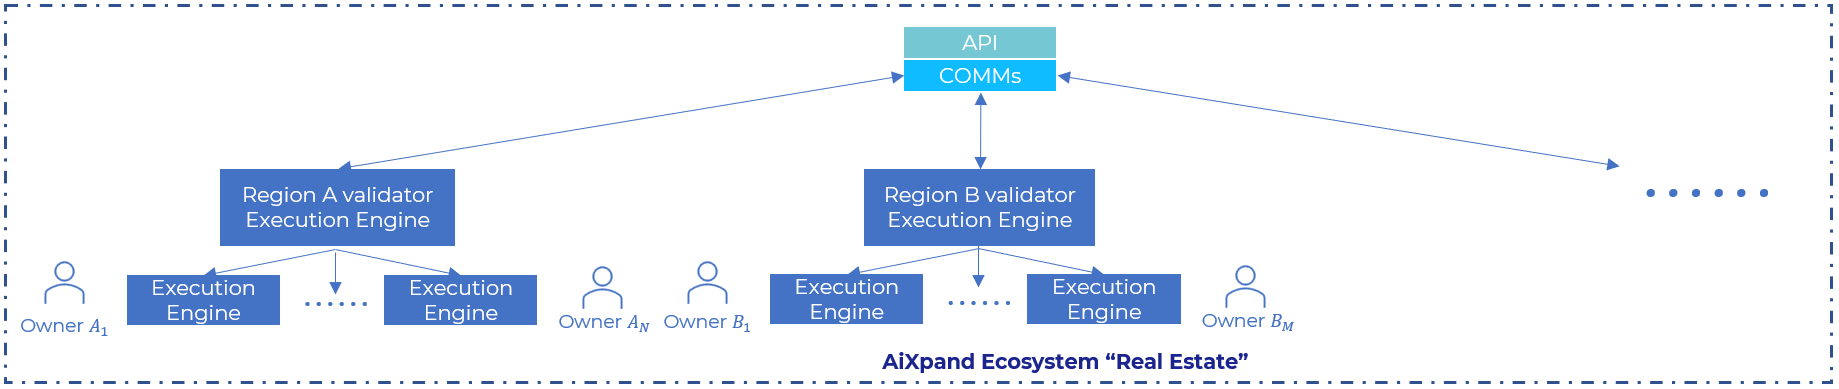
\includegraphics[width=16cm]{aixp_overall.png}
    \caption{\textit{Overall view of the AiXpand execution engines network-of-networks}}
    \label{fig:aixp_overall}
\end{figure}


In \figurename{\ref{fig:aixp_overall}} the regional "validation" nodes coordinate the communication between nearby local nodes as well as provide inter-region distributed ledger data sync.

[TEXT]


\begin{figure}[h]
    \centering
    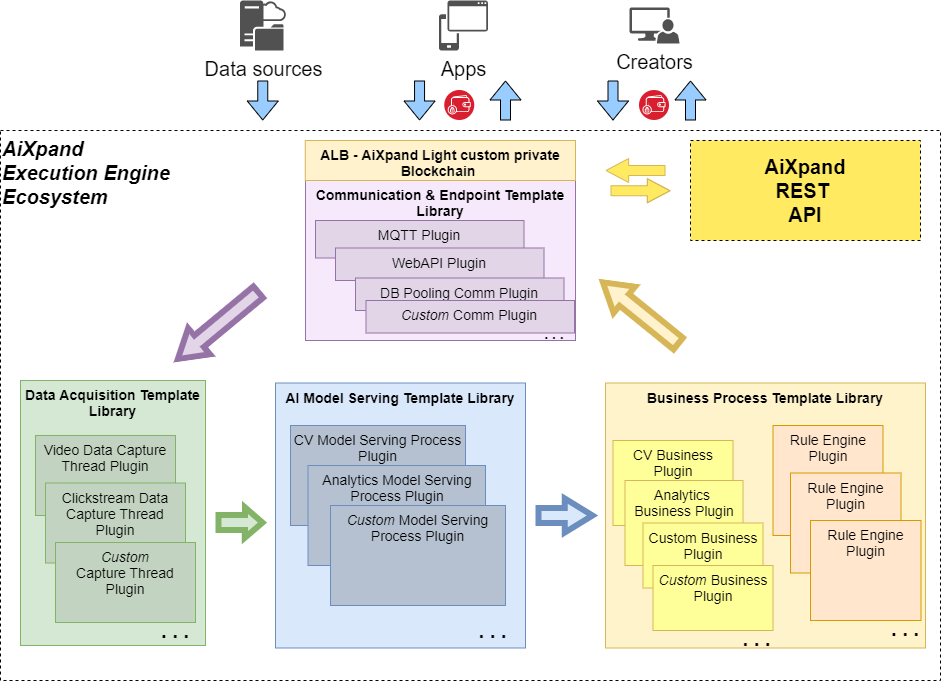
\includegraphics[width=16cm]{ee.png}
    \caption{\textit{Top view of AiXpand Execution Engine ecosystem}}
    \label{fig:ee}
\end{figure}


In order to summarize the funds allocation and distribution in our job execution agnostic reward pools we will denote $T_{N}$ as the lifetime total time the given \textit{Node} $N$, identified by a unique smart-contract based \textit{Node Deed}, has been alive in the network; $T_{epoch}$ as the protocol epoch time - the time interval used to calculate and distribute a round of rewards to all active nodes, $E$ as the total number of epochs since the protocol \textit{genesys}, $P_{N_E}$ the power index of a given node $N$ during epoch $E$. The final formula of the reward $R_{N_E}$ of the $Node$ $N$ at epoch $E$ is presented in below \equationautorefname{\ref{eqr:5}} 

\begin{align}
A_{N_{E}} &= \frac {T_{Node}}{T_{epoch} * N_E}\label{eqr:1}\\
F_{E} &=\sum_{X}{P_{X_E} * T_{X}}\label{eqr:2}\\
I_{N_E} &= e^{P_{N_E} * A_{N_{E}}}\label{eqr:3}\\
I_{E} &= e^{F_{E}}\label{eqr:4}\\
R &= \frac{I_{N_E}}{I_{E}} \label{eqr:5}
\end{align}



\subsection{End-to-end low-code pipelines - R}
Text
\subsection{Custom secure execution and the Plugin API}

Due to the nature of trust-less decentralized distributed job execution multiple security issues arise such as (a) custom code safety, (b) request and result message immutability, (c) data confidentiality and (d) solution proofing. While later three are cryptography related issues solved either by our proposed internal distributed ledger architecture including zero-knowledge proofing or by employing neural model training and inference based on homomorphic encryption, the former proposed solution rely on code safety checking and signing.

Two main categories of \emph{business} plugins have been created - secure and user plugins - currently based on Python\cite{vanrossum1995python} high-level general-purpose programming language. While the former plugins are either plugins that can be either considered generic templates or \emph{default} \emph{business insights} data/report preparation plugins the later are ranging from user plugins deployed as proposals for future secure services up to \emph{code pieces} written by anyone using the execution engine within the trust-less network. Both the deployed user plugins as well as the custom user \emph{code pieces} are considered potentially unsafe by their nature and thus (a) limited in terms of programming language keywords, functions and packages to a specific higher level \emph{Plugin API} and (b) hash-sign verified, profiled and code re-checked for code-injection and other tampering processes each time a distributed execution is requested. To further impose custom \emph{user} code execution safety this behaviour is imposed both then a code is peer-to-peer transferred and executed remotely as well as when the initiator is the same as the worker.

\subsection{Multi-framework serving processes - R/WPI}
Text - paragraph tf, th, anything - isolated and monitored plugin-processes

\subsection{Distributed decentralized execution -S/WPI}
Text

+ basic map-reduce algo (referenced)

\subsection{Integration with Web3 Radu/WIP}

\textbf{[Gentle intro needed]}

There are 2 stages for any request made on the AiXpand network and the purpose of the API is to automate and handle the lifecycle of the request. The first stage is the financial one which involves committing to an amount of tokens to be spent on the AI request. The second is the actual call to the AiXpand network with the transaction details attached. In order to minimize the cryptocurrencies networks’ costs, it is possible to commit a larger amount in an escrow account and allow the AiXpand internal blockchain to keep track of the spent funds.

Depending upon implementation, the API library will leverage specific web3 components for interacting with the payment channels. On the execution engine side, a simple check is made: either the request is signed by the node owner and is to be run locally, in which case no payment is necessary, or a valid funding transaction has been attached.

The purpose of AiXpand API is to handle all the necessary financial details before publishing the request on the network and to abstract this part away in order to facilitate an easy integration in third party systems.

The second stage is a simple message published to the nearest validator node or the user’s owned node. From this point forward the request will be handled by the network.

TODO: describe calls to AiXpand network and provide a high level impl


AID TEXT referencing text1 \ref{alg:rewards}  text2 \ref{alg:jobexec}  text3 \ref{alg:joballoc}


\section{Applications}

Text - short intro by AID / WIP

\subsection{Physical security \& safety - Bleo/wip}
The average attention span of a human is somewhere around 10 seconds and that decreases when a single operator has to constantly be aware of what happens in 10, 15 or even 20 video streams. Observing this we can conclude that the use of machine learning in video surveillance is a major breakthrough.
		    
When the operator is assisted by several machine learning algorithms designed to detect several unusual events, its job becomes considerably easier.
We will further categorize the use-cases in: industrial personal safety, location security and video equipment security.

\begin{itemize}
    \item {Industrial personal safety (based on analyzing people's posture and body positioning)

    We will use a multiple-stage machine learning model and potential heuristics in order to classify the human participants in a given scene.
    }
    By firstly using a YOLO model to localize all the persons in the scene we, then, will be using a MSPN model to localize each person's body parts(e.g. left eye, mouth, right leg etc.).
    Based on the person's posture we can infer several things.
    \item {Location security (based on analyzing the appearence of either humans, animals or even certain objects in a given scene)}
    \item {Video equipment security (based on analyzing the image quality and the scene itself in order to detect potential damage suffered by the recording equipment either by natural causes or by human intervention)}

\end{itemize}
    \subsubsection{Use-cases}
    Default pipelines
        \paragraph{Industrial personal safety}
        Text
        \paragraph{Location security}
        Text
        \paragraph{Video equipment security}
        Text


\subsection{Predictive analytics - R}
Predictive analytics is the use of data, statistical algorithms and machine learning techniques to identify the likelihood of future outcomes based on historical data \cite{klimberg2016fundamentals}. Such techniques are used by a large variety of businesses - from retail brick and mortar stores to physical security companies in order to optimize their business processes or to make predictions regarding the future behaviour of people or equipment.

\subsubsection{Use-cases: Predictive replenishment - Razvan + Radu}

\paragraph{Replenishment - Draft} One of the biggest problems of retail logistics is that of over-supply and under-supply. Oversupply can incur losses based on the perishability of the over-supplied products, as it is not sold in time and based on the fact that it's storage also costs; while under-supply induce missed potential sales as the under-supplied product is not in stock

The easiest, but not the most efficient solution is the use of heuristics \cite{stefanovic2015collaborative} to generate replenishment orders. The main drawback is that good results require very complex heuristics which are hard to maintain and do not easily scale. The alternative to the heuristic method is the automated learning approach. Machine learning techniques, especially deep representation models \cite{kilimci2019improved}, are able to accurately find patterns in historical data and using continuous training methods can easily adapt to new circumstances in order to provide reliable consumption predictions.

\paragraph{A simple use-case Excel} Text text

\subsubsection{Predictive maintenance - Razvan/WiP}
The problem of predictive maintenance seeks to preemptively address points of failure in industrial equipment before critical malfunctions appear \cite{mobley2002introduction}. Equipment breakdown can be predicted, and thus averted, by monitoring slight changes in its behaviour and correlating them with the historical comportment of similar items.

The common solution, similar to the replenishment problem, is the employment of heuristics with the purpose of scheduling equipment maintenance. Same as in the replenishment case, heuristics based approaches do not scale to a large number of conditions, have low accuracy and are hard to maintain. As a consequence, deep learning based methods \cite{zhao2019deep} need to be employed in order to have an accurate and scalable system. Deep models can reliably identify patterns and predict future malfunctions and easily generalize to new circumstances in order to provide a reliable solution.


\subsubsection{Anomaly detection - Razvan/Draft}
Anomaly detection is the task of detection and identification of data points that deviate from the majority of the data \cite{chandola2009anomaly}. It can be employed in physical security applications in order to identify possible security threats or system malfunctions. Such systems are needed because the large volume of telemetry and events are expensive to be parsed by human operators and are prone to errors due to the tedious nature of the task. 

A frequent solution to the anomaly detection problem is use of multivariate gaussian models in order to identify suspect events \cite{mehrotra2017anomaly}. This method has low computational cost, is easy to implement but has low accuracy and it can not represent and take advantage of complex patterns in the data. An alternative is the employment of deep representation models \cite{chalapathy2019deep} such that higher order patterns can be made use of. 


\subsection{Motionmask \texttrademark ----- Radu + Narcis + Beatrice}
Motionmask is the first product built and launched end-to-end in the AiXPAND ecosystem. Motionmask is a desktop and mobile web application which blurs videos with the goal of achieving further privacy-compliant video processing.
\subsubsection{Online video anonymization}
At the core of Motionmask lie very powerful AI detection models. These models require a lot of computing resources which, since Motionmask is an online available tool, would have to be provided solely by Motionmask itself. This would not be possible and efficient without the AiXpand ecosystem because it would require for Motionmask to have an infrastructure small enough to avoid wastage but also big enough to support big spikes and not let Motionmask users down. 
\subsubsection{Focus on front-end}
Text

\subsection{Other applications}
\subsubsection{Gaming - Bleo and Stefan / WIP}
 - Objectives \& approach
 - A simple life-game


\section{Conclusions \& ongoing work}
Text
\subsection{Distributed homomorphic encryption}
Text
\subsubsection{Training}
Text
\subsubsection{Inference}
Text

\subsection{Two layers of BC}
Text

\subsection{Oracles between on-chain and Execution Engines worlds}
Text

\subsection{Zero Knowledge proofs}
Text

%Bibliography
\bibliographystyle{unsrt}  
\bibliography{references}  


\begin{algorithm}
\caption{\textit{\textbf{AiXpRewards} - generic \textbf{AiXpand} reward allocation end-to-end protocol}}\label{alg:rewards}
\textbf{Data/Inputs:}\vspace{1mm}\\
\hspace*{5mm} $N$  \Comment{N is the maximum number of nodes allowed by the protocol}\vspace{1mm}\\
\hspace*{5mm} $BC$ \Comment{\textit{Layer 1} or \textit{Layer 2} online block-chain protocol that will enable micro-transactions}\\
\hspace*{5mm} $EscrowPool$  \Comment{a \textit{smart-contract} in \textit{BC} holding unfinished jobs funds}\vspace{1mm}\\
\hspace*{5mm} $RewardPool$  \Comment{a \textit{smart-contract} in \textit{BC} holding finished jobs funds}\vspace{1mm}\\
\hspace*{5mm} $NodeDeeds[N]$ \Comment{The list of \textit{non-fungible} node-deed \textit{smart contracts} living in \textit{BC}}\vspace{1mm}\\
\hspace*{5mm} $MaxEpochTime$  \Comment{Seconds in a AiXpand epoch }\vspace{1mm}\\
\hspace*{5mm} $Initialize$  \Comment{Initializes all smart-contracts}\vspace{1mm}\\
\hspace*{5mm} $MaybeUpdate$  \Comment{Updates (async and parallel) node deeds smart contracts using \textit{BC}}\vspace{1mm}\\
\hspace*{5mm} $CurrentTime$  \Comment{Seconds from 2000 or similar function}\vspace{1mm}\\
\hspace*{5mm} $GetNewJob$  \Comment{Generic function that retrieves a job data from posted jobs list.}\\
\hspace*{5mm} 
\begin{algorithmic}[1]
    \State $ProtocolState \gets GENESYS$ \Comment{This is the initial protocol \textit{genesys} stage}\;\vspace{1mm}
    \State $NodeDeeds \gets$ \textbf{call} $Initialize(BC)$\; \Comment{All deeds are initialized, although not all are distributed initially}\vspace{1mm}
    \State $AiXpEpoch \gets 0$;\vspace{1mm}
    \State $EscrowPool \gets 0;$\vspace{1mm}
    \State $RewardPool \gets 0;$\vspace{1mm}
    \State $ProtocolState \gets PROCESSING$; \Comment{We start distributing jobs and rewards stage}\;\vspace{1mm}
    \While{$True$}\vspace{1mm}
        \State $AiXpEpoch \gets AiXpEpoch + 1$;\vspace{1mm}
        \State $NodeDeeds \gets$ \textbf{call} $MaybeUpdate(BC)$;\vspace{1mm} \Comment{Allocation of deeds happening in other algo}\vspace{1mm}
        \State $StartTime \gets CurrentTime()$;\vspace{1mm}
        \While{$(CurrentTime() - StartTime) < MaxEpochTime$}\vspace{1mm}
            \While{$NewJobData \gets GetNewJob(BC)$} \textbf{\textit{in parallel}}\vspace{1mm}
                \State $Job, JobReward, Sender \gets NewJobData$;\vspace{1mm}\Comment{Job info is already available in BC}\vspace{1mm}
                \State $EscrowPool \gets EscrowPool + JobReward$;\vspace{1mm}
                \State \textbf{call async \textit{AiXpExecCheck}}\textit{(Job, JobReward, Sender)}; \ref{alg:jobexec}\vspace{1mm}
            \EndWhile\vspace{1mm}
        \EndWhile\vspace{1mm}
        \State $ActiveNodes \gets$ \textbf{call} $AiXpGetCurrentEpochNodeStatus()$;\vspace{1mm}
        \State $currNode \gets 0$;\vspace{1mm}
        \While{$RewardsPool > 0$}\; \Comment{\textit{RewardsPool} will be fully distributed among all participants }\vspace{1mm}
            \State $EpochActiveTime, EpochActivePower \gets ActiveNodes[currNode]$;\vspace{1mm}
            \State $currRewardPrc \gets \textbf{\textit{AiXpAlloc}}(currNode)$\ref{alg:joballoc};\vspace{1mm}
            \State $currReward \gets RewardsPool * currRewardPrc$;\vspace{1mm}
            \State $RewardsPool \gets RewardsPool - currReward$;\vspace{1mm}
            \State $NodeDeeds[currNode].addFunds(currReward)$;\vspace{1mm}
            \State $currNode \gets currNode + 1$;\vspace{1mm}
        \EndWhile
    \EndWhile\vspace{1mm}
\end{algorithmic}
\end{algorithm}

\begin{algorithm}
\caption{\textit{\textbf{AiXpExecCheck} - generic \textbf{AiXpand} execution \& escrow release}}\label{alg:jobexec}
\textbf{Inputs:}\\
\hspace*{5mm} $Job$  \Comment{the \textit{job} request that will be distributed in the decentralized network}\vspace{1mm}\\
\hspace*{5mm} $JobReward$  \Comment{the proposed job fee payed by the \textit{Sender} of the job}\vspace{1mm}\\
\hspace*{5mm}  \Comment{Assumption is that the \textit{JobReward} has been already allocated in the \textit{EscrowPool}}\vspace{1mm}\\
\hspace*{5mm} $Sender$  \Comment{the \textit{owner} of the job request}\vspace{1mm}\\
\textbf{Data:}\\
\hspace*{5mm} $EscrowPool$  \Comment{a \textit{smart-contract} in \textit{BC} holding unfinished jobs funds}\vspace{1mm}\\
\hspace*{5mm} $RewardPool$  \Comment{a \textit{smart-contract} in \textit{BC} holding finished jobs funds}\vspace{1mm}\\
\hspace*{5mm} $JobStatus$  \Comment{a on-chain \textit{smart-contract} based matrix of jobs per \textit{Node}}\vspace{1mm}\\
\hspace*{5mm} $JobCount$  \Comment{a on-chain \textit{smart-contract} based vector of ongoing jobs per Node}\vspace{1mm}\\
\begin{algorithmic}[1]
    \State $JobCount[Sender] \gets JobCount[Sender] + 1$;\vspace{1mm}
    \State $JID \gets JobCount[Sender]$;\vspace{1mm}
    \State $JobStatus[Sender][JID] \gets IN\_PROGRESS$;\vspace{1mm} \Comment{JobStatus is stored in a on-chain smart-contract}
    \While{$JobStatus[Sender][JID] == IN\_PROGRESS$}\vspace{1mm}
        \If {$Job.Status != NULL$}\vspace{1mm}
        \State $JobStatus[Sender][JID] \gets Job.Status$;\vspace{1mm}
        \EndIf\vspace{1mm}
    \EndWhile\vspace{1mm}
    \If {$Job.Status == DONE$}\vspace{1mm}
        \State $EscrowPool \gets EscrowPool - JobReward$;\vspace{1mm}
        \State $RewardsPool \gets RewardsPool + JobReward$;\vspace{1mm}        
    \Else\vspace{1mm}
        \State $EscrowPool \gets EscrowPool - JobReward$;\vspace{1mm}
        \State \textbf{call} $LockFundsForReview(Job, JobReward, TIME\_24H);$ \Comment {Funds locked pending review}\vspace{1mm}
    \EndIf\vspace{1mm}
    \State $JobStatus[Sender][JID] \gets NULL$;\Comment{Reset onchain storage data}\vspace{1mm}
\end{algorithmic}
\end{algorithm}

\begin{algorithm}
\caption{\textit{\textbf{AiXpAlloc} - generic \textbf{AiXpand} Node pool-share allocation}}\label{alg:joballoc}
\textbf{Inputs:}\\
\hspace*{5mm} $currNodeDeed$  \Comment{\textit{smart-contract} based unique identifier of the AiXpand processing Node to be rewarded}\vspace{1mm}\\
\textbf{Data:}\\
\hspace*{5mm} $MaxEpochTime$  \Comment{Seconds in a AiXpand epoch }\vspace{1mm}\\
\hspace*{5mm} $A$  \Comment{list of all Active Nodes based on oracle stored in a on-chain \textit{smart-contract}}\vspace{1mm}\\
\hspace*{5mm} $RewardPool$  \Comment{\textit{smart-contract} of the reward pool that acts as a escrow account}\vspace{1mm}\\
\begin{algorithmic}[1]
    \State $AlivePrc \gets A[currNodeDeed].totalAliveTime / (MaxEpochTime * AiXpEpoch)$;\vspace{1mm}
    \State $Power \gets A[currNodeDeed].power$;\Comment{Either capacity or actual}\vspace{1mm}
    \State $NPI \gets Power * AlivePrc$;\Comment{the Node Power Index is calculated}\vspace{1mm}
    \State $FP \gets \sum_{X in A} {X.Power * X.AlivePrc}$;\Comment{the full network power index is calculated}\vspace{1mm}
    \State $R \gets \frac{e^{NPI}}{e^{FP}}$\vspace{1mm}
    \State \textbf{return} $R$
\end{algorithmic}
\end{algorithm}
\end{document}
